\section{Desafio}

\begin{minipage}{\linewidth}
  \centering
  \begin{minipage}{0.45\linewidth}
    Dado o circuito da \textbf{Figura \ref{fig:CircuitoDesafio}},
    considerar: $R_1 = 330\Omega$,
                $R_2 = 150\Omega$,
                $R_3 = 270\Omega$, \\
                $R_4 = 400\Omega$ e
                $R_5 = 100\Omega$.
    \begin{itemize}
      \item Identificar:
      \begin{itemize}
        \item os nós do circuito;
        \item a configuração de ligação dos componentes: série ou paralelo;
      \end{itemize}
      \item Calcular a resistência equivalente em cada ramo;
      \item Simplificar o circuito ao redesenhá-lo;
      \item Repetir o processo até obter a resistência equivalente total.
    \end{itemize}
  \end{minipage}
  \hspace{0.05\linewidth}
  \begin{minipage}{0.45\linewidth}
    \begin{figure}[H]
      \centering
      \caption{Circuito elétrico misto}
      \label{fig:CircuitoDesafio}
      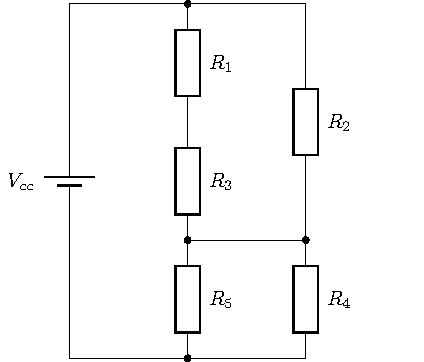
\includegraphics[scale=1.0]{fig-desafio}

      {\small Fonte: Próprio autor.}
    \end{figure}
  \end{minipage}
\end{minipage}
